
%(BEGIN_QUESTION)
% Copyright 2006, Tony R. Kuphaldt, released under the Creative Commons Attribution License (v 1.0)
% This means you may do almost anything with this work of mine, so long as you give me proper credit

Examine the following four-electrode conductivity analyzer circuit, then answer the questions that follow:

$$\includegraphics[width=15.5cm]{i00910x01.eps}$$

\begin{itemize}
\item{} If the current source's output were to increase, would $V_{out}$ {\it increase}, {\it decrease}, or {\it stay the same}?
\vskip 5pt
\item{} If the conductivity of the liquid were to increase, would $V_{out}$ {\it increase}, {\it decrease}, or {\it stay the same}?
\vskip 5pt
\item{} If the two outer electrodes (connected to the current source) were to become plated with minerals or some other non-conducting coating, would $V_{out}$ {\it increase}, {\it decrease}, or {\it stay the same}?
\vskip 5pt
\item{} If the sampled liquid is tap water, identify something you could do to the water to increase its conductivity.
\end{itemize}

\underbar{file i00910}
%(END_QUESTION)





%(BEGIN_ANSWER)

\begin{itemize}
\item{} If the current source's output were to increase, $V_{out}$ would {\bf increase}.
\vskip 5pt
\item{} If the conductivity of the liquid were to increase, $V_{out}$ would {\bf decrease}.
\vskip 5pt
\item{} If the two outer electrodes (connected to the current source) were to become plated with minerals or some other non-conducting coating, $V_{out}$ would {\bf stay the same}.
\vskip 5pt
\item{} You could add salt or some other ionic compound to the water to increase its conductivity.  You could also heat the water to a greater temperature.
\end{itemize}

%(END_ANSWER)





%(BEGIN_NOTES)

$$\includegraphics[width=15.5cm]{i00910x02.eps}$$

\vskip 20pt \vbox{\hrule \hbox{\strut \vrule{} {\bf Virtual Troubleshooting} \vrule} \hrule}

This question is a good candidate for a ``Virtual Troubleshooting'' exercise.  Presenting the diagram to students, you first imagine in your own mind a particular fault in the system.  Then, you present one or more symptoms of that fault (something noticeable by an operator or other user of the system).  Students then propose various diagnostic tests to perform on this system to identify the nature and location of the fault, as though they were technicians trying to troubleshoot the problem.  Your job is to tell them what the result(s) would be for each of the proposed diagnostic tests, documenting those results where all the students can see.

During and after the exercise, it is good to ask students follow-up questions such as:

\begin{itemize}
\item{} What does the result of the last diagnostic test tell you about the fault?
\item{} Suppose the results of the last diagnostic test were different.  What then would that result tell you about the fault?
\item{} Is the last diagnostic test the best one we could do?
\item{} What would be the ideal order of tests, to diagnose the problem in as few steps as possible?
\end{itemize}

%INDEX% Measurement, analytical: conductivity

%(END_NOTES)


